\documentclass[compress,12pt]{beamer}


%\usepackage{newtxtext,newtxmath} % Times moderne pour texte et maths

% -------------------------------------
% Paquets utiles
% -------------------------------------
\let\Bbbk\relax
\let\openbox\relax
\usepackage[french]{babel}
\usepackage{amsmath, amssymb, amsthm}
\usepackage{xcolor}
\usepackage{bm}
\usepackage{braket}


%\usepackage{media9}
%\usepackage{media4pdf}
\usepackage{graphicx}
\usepackage{animate}

\usepackage{tikz}  % charger TikZ d'abord
\usetikzlibrary{arrows.meta, positioning, shapes} % puis les libraries nécessaires

\usetikzlibrary{animations} % LaTeX and plain TeX
\usetikzlibrary{decorations.markings}

\usetikzlibrary{decorations.text}

%\usepackage{fontspec} % utiliser xelatex/lualatex
%\usepackage[T1]{fontenc}
\usepackage{calligra}  % jolie police cursive
\usepackage{xcolor}

% === Définir les couleurs ===
\definecolor{fondgris}{HTML}{212529}
\definecolor{blanc}{RGB}{255,255,255}

% === Commande pratique ===
\newcommand{\calitext}[1]{{\calligra\fontsize{36}{40}\selectfont #1}}

% Commandes pour les flèches textuelles
% Désactive les shorthands dans TikZ
\AtBeginDocument{\shorthandoff{:;!?}}
\tikzset{every picture/.style={execute at begin picture={\shorthandoff{:;!?};}}}
\tikzstyle{every picture}+=[remember picture]
\tikzstyle{na} = [shape=rectangle,inner sep=0pt]


\newcommand{\ptFleche}[2]{		% Déclaration d'une extrémité de flèche
    \shorthandoff{:;!?}% <- désactive les shorthands
    \tikz[baseline=(#1.base)]\node[na](#1){#2};
  }

\newcommand{\Fleche}[5][thick]{%
    \begin{tikzpicture}[overlay]
        \path[->,#1](#2) edge [out=#4, in=#5] (#3);
    \end{tikzpicture}
}

% --- Commande FlecheEllipse ---
% #1 = nœud source (nom)
% #2 = angle sortie du nœud source
% #3 = angle entrée du nœud cible
% #4 = décalage dx, dy sous forme (dx,dy) en cm
% #5 = couleur ellipses et flèche
% #6 = texte du nœud cible B
\newcommand{\FlecheEllipseo}[6]{%
    \begin{tikzpicture}[overlay, remember picture]
        % Coordonnées source
        \path let \p1 = (#1) in 
        coordinate (Acoord) at (\x1,\y1);

        % Coordonnées cible
        \pgfmathsetmacro{\dx}{#4}
        \pgfmathsetmacro{\dy}{#5} % ici on sépare les deux pour le calcul

        \coordinate (B) at ([shift={(#4)}]#1);

        % Nœud A entouré d'ellipse
        \node[draw,#5,ellipse,inner sep=2pt] (#1-node) at (#1) {#1};
        % Nœud B entouré d'ellipse
        \node[draw,#5,ellipse,inner sep=2pt] (B-node) at (B) {#6};
        % Flèche de A vers B
        \draw[->,#5,thick] (#1-node) edge [out=#2,in=#3] (B-node);
    \end{tikzpicture}%
}

% --- Commande FlecheEllipse finale ---
% #1 = nom du nœud source (A)
% #2 = angle sortie du nœud source
% #3 = angle entrée du nœud cible
% #4 = décalage horizontal dx (en cm)
% #5 = décalage vertical dy (en cm)
% #6 = couleur ellipses et flèche
% #7 = contenu du nœud B (texte, formule, TikZ, etc.)
\newcommand{\FlecheEllipse}[7]{%
    \begin{tikzpicture}[overlay]
        % --- Nœud source A ---
        \node[draw,#6,ellipse,inner sep=2pt](#1){};

        % --- Nœud cible B ---
        \coordinate (B) at ($(#1) + (#4cm,#5cm)$);
        \node[draw,#6,ellipse,inner sep=2pt] (B-node) at (B) {#7};

        % --- Flèche de A vers B ---
        \draw[->,#6,thick] (#1) edge [out=#2,in=#3] (B-node);
    \end{tikzpicture}%
}
%%%%%%%%%%%%%%%%%%%%%%%%%%%%%%%%%%
\newcommand{\operatorvec}[1]{\vec{{\bm{#1}}}} % pour les operateur
\newcommand{\operator}[1]{\hat{\bm{#1}}} % pour les operaeur vecteur
\newcommand{\operatormat}[1]{\operatorname{#1}} % pour les operaeur vecteur
\newcommand{\operatortilde}[1]{\tilde{\bm{#1}}} % pour les opetateur avec un tilde
\newcommand{\operatortildevec}[1]{\tilde{\bm{#1}}}% pour les opetateur avec un tilde et vecteur
\newcommand{\dfonc}[1]{\mathscr{D}_{[#1]}}
%%%%%%%%%%%%%%%%%%%%%%%%%%%%%%%%%%

\usetheme{Arguelles}
% \usetheme{Madrid}
% \usecolortheme{default}

\title{Study \\ 
       of the out-of-equilibrium dynamics \\
       of \mbox{one-dimensional Bose gases}}
\subtitle{Étude de la dynamique hors équilibre des gaz de Bosons unidimensionnels}
\event{}
%\venue{}
\date{04-11-2025}
\author{Guillaume THÉMÈZE}
\institute{Université Paris-Saclay \\ Laboratoire Charles Fabry}
%\email{guillaume.themeze@institutoptique.fr}
%\homepage{www.mywebsite.com}
%\github{THEMEZE}

\begin{document}

\frame[plain]{\titlepage}

\Section{Introduction}

% Team 
% \begin{frame}
%   \frametitle{Team}
%   %\framesubtitle{Subtitle here}
%   \centering
%   
\includegraphics[width=0.6\linewidth , page = 1 ]{figures/Figures_temporaire.pdf}
     
% \end{frame}

% Rapidities and GGE in a classical system
\begin{frame}
  \frametitle{Rapidities and GGE in a classical system}
  
  %\begin{columns}
  
    % === Colonne gauche ===
    %\begin{column}{0.5\textwidth}
      \begin{columns}[T, totalwidth=\textwidth]
        \centering
        \begin{column}{0.5\textwidth} 
          \centering
          \begin{block}{Chaotic/Ergodic}
          \end{block}
        \end{column}
        \begin{column}{0.5\textwidth} 
          \centering
          \begin{block}{Integrable/non-ergidic}
          \end{block}
        \end{column}
      \end{columns}

      \begin{columns}[c, totalwidth=\textwidth]
      
        % --- Sous-colonne gauche ---
        \begin{column}{0.5\textwidth} 
          \centering
          %\begin{block}%{Chaotic/Ergodic}\centering
          \animategraphics[
            %controls, 
            %autoplay, % démarre automatiquement 
            %loop, % boucle infinie,
            %palindrome, % (optionnel) rejoue à l'envers,
            %clicktoshow, % permet de lancer/pause par clic
            width=0.6\linewidth,
            buttonsize=1em,
            poster=first
          ]{60}{figures/frames_2D_positions_animation/frame_}{00001}{00001}

          {\fontsize{10}{5}\selectfont 
          \begin{tikzpicture}[remember picture, overlay]
            \node []  at  (2,2.5)   (part)                            {$n$};
            \node []     (moment) [below=1mm of part]             {$nu$};
            \node []     (nrj) [below=1mm of moment]             {$\varepsilon$};
	          \draw[  opacity = 0.5 ]
		          (part) edge[line width=0.2ex ,color = blue ,arrows = {Computer Modern Rightarrow[sharp ,length=0.2cm]-},  , out = 90 , in = 180  ]node[pos=1, right]{\color{blue} \fontsize{6}{1}\selectfont \bfseries  particule density }($(part) + (1cm,1.0cm)$)
              (moment) edge[line width=0.2ex ,color = red ,arrows = {Computer Modern Rightarrow[sharp ,length=0.2cm]-},  , out = 0 , in = 180  ]node[pos=1, right]{\color{red} \fontsize{6}{1}\selectfont \bfseries  velocity maen }($(moment) + (1cm,0cm)$)
              (nrj) edge[line width=0.2ex ,color = black ,arrows = {Computer Modern Rightarrow[sharp ,length=0.2cm]-},  , out = -90 , in = 180  ]node[pos=1, right]{\color{black} \fontsize{6}{1}\selectfont \bfseries  energie density }($(nrj) + (1cm,-1.0cm)$)
	          ;
          \end{tikzpicture}
          }
        %\end{block}
        \end{column}
        
        % --- Sous-colonne droite ---
        \begin{column}{0.5\textwidth} 
          \centering
          %\begin{block}%{Integrable/non-ergidic}\centering
          
          \animategraphics[
            width=0.6\linewidth,
            buttonsize=1em,
            poster=first
          ]{60}{figures/frames_1D_positions_animation/frame_}{00001}{00001} 

          {
          \fontsize{10}{5}\selectfont 
          \begin{tikzpicture}[remember picture, overlay]
            \node []  at  (0,0)   (rho)                            {$\rho(v)$};
	          \draw[  opacity = 0.5 ]
              (rho) edge[line width=0.2ex ,color = black ,arrows = {Computer Modern Rightarrow[sharp ,length=0.2cm]-},  , out = -90 , in = 180  ]node[pos=1, right]{\color{black} \fontsize{6}{1}\selectfont \bfseries  velocity density }($(rho) + (1cm,-1.0cm)$)
	          ;
          \end{tikzpicture}
          }
          
          
        %\end{block}
        \end{column}
        
      \end{columns}
    %\end{column}
    \vspace{0.2cm}
    % === Colonne droite ===
   %\begin{column}{0.5\textwidth} 
      \begin{columns}[T, totalwidth=\textwidth]
      
        % --- Sous-colonne gauche ---
        \begin{column}{0.5\textwidth} 
          \centering
          \begin{block}{}
          \centering
          \begin{columns}[c, totalwidth=\textwidth]
            \begin{column}{0.4\textwidth} 
              \centering
              \animategraphics[
                width=1.0\linewidth,
                buttonsize=1em,
                poster=first
              ]{60}{figures/frames_2D_velocity_distribution/frame_}{00001}{00001}
           \end{column}
           \begin{column}{0.2\textwidth} 
            \centering
            {\fontsize{6}{5}\selectfont 
            $$ \overset{thermalisation}{\Longrightarrow} $$
            }
           \end{column}
           \begin{column}{0.4\textwidth} 
              \centering
              \animategraphics[
                width=1.0\linewidth,
                buttonsize=1em,
                poster=first
              ]{60}{figures/frames_2D_velocity_distribution/frame_}{00600}{00600}
            \end{column}
          \end{columns}
          \end{block}
        \end{column}
        
        % --- Sous-colonne droite ---
        \begin{column}{0.5\textwidth} 
          \centering
          %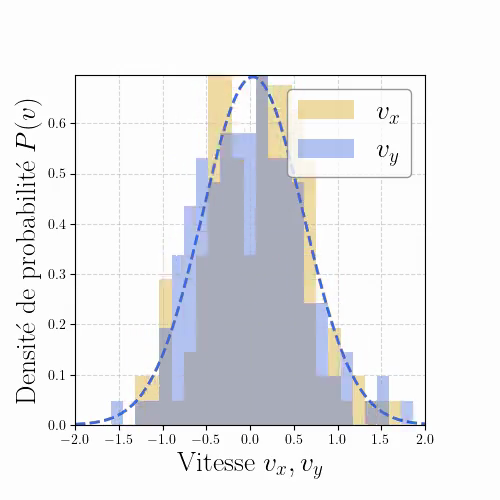
\includegraphics[width=0.6\linewidth]{figures/frames_2D_velocity_distribution/frame_00600.png}
          \animategraphics[
            width=0.5\linewidth,
            buttonsize=1em,
            poster=first
          ]{60}{figures/frames_1D_velocity_distribution/frame_}{00001}{00001} 
        \end{column}
        
      \end{columns}
    %\end{column}
    
  %\end{columns}

\end{frame}

%How do you make 1D?
% \begin{frame}
%   \frametitle{How do you make 1D?}
  
%   %\begin{columns}
  
%     % === Colonne gauche ===
%     %\begin{column}{0.5\textwidth}
%       \begin{columns}
      
%         % --- Sous-colonne gauche ---
%         \begin{column}{0.5\textwidth} 
%           \centering
%           
\includegraphics[width=0.6\linewidth , page = 2 ]{figures/Figures_temporaire.pdf}
%         \end{column}
        
%         % --- Sous-colonne droite ---
%         \begin{column}{0.5\textwidth} 
%           \centering
%           
\includegraphics[width=0.6\linewidth , page = 3 ]{figures/Figures_temporaire.pdf}
%         \end{column}
        
%       \end{columns}
%     %\end{column}
%     \vspace{0.2cm}
%     % === Colonne droite ===
%     %\begin{column}{0.5\textwidth} 
%       \begin{columns}
      
%         % --- Sous-colonne gauche ---
%         \begin{column}{0.5\textwidth} 
%           \centering
%           
\includegraphics[width=0.6\linewidth , page = 4 ]{figures/Figures_temporaire.pdf}
%         \end{column}
        
%         % --- Sous-colonne droite ---
%         \begin{column}{0.5\textwidth} 
%           \centering
%           
\includegraphics[width=0.6\linewidth , page = 5 ]{figures/Figures_temporaire.pdf}
%         \end{column}
        
%       \end{columns}
%     %\end{column}
  
%   %\end{columns}

% \end{frame}

% Thesis Problematic
\begin{frame}
  \frametitle{Thesis Problematic}
  %\scalebox{1.0}{
  \begin{columns}[T, totalwidth=\textwidth]
    \begin{column}{0.9\textwidth}
      {\fontsize{10}{12}\selectfont  % <- ajuste ici aussi
      \begin{block}{Scientific Question}
        How can we characterize the spatio-temporal evolution of a 1D quantum gas after a perturbation, 
        in terms of the local rapidity distribution and its link to Generalized Gibbs Ensembles (GGE)?
      \end{block}
      }
    \end{column}
    \begin{column}{0.1\textwidth}
      {~}
    \end{column} 
  \end{columns}
  
  \vspace{0.2cm}

  \begin{columns}[c, totalwidth=\textwidth]

     % --- Left column: illustration ---
    \begin{column}{0.4\textwidth}
      \centering
      
\includegraphics[width=\textwidth , page = 6 ]{figures/Figures_temporaire.pdf}
      \vspace{0.2cm}

      %\small
      %\emph{Schematic view: from experimental system to theoretical description.}
    \end{column}

    % --- Right column: text ---
    \begin{column}{0.58\textwidth}
      {\fontsize{10}{12}\selectfont  % <- ajuste ici aussi
      \begin{block}{Objectives}
        \begin{itemize}
          \item Lieb and Liniger;
          \item GHD;
          \item Manip;
          \item Bipartition;
          \item Fluctuation 
        \end{itemize}
      \end{block}
      }
    \end{column}
    
  \end{columns}
  %}
\end{frame}

\Section{Lieb-Liniger}

%The 2-body problem: the scattering phase
% \begin{frame}
%   \frametitle{The 2-body problem: the scattering phase}
%   %\framesubtitle{Shift collisionnel 2 corps BA}
%   \begin{columns}[c, totalwidth=\textwidth]
%     \begin{column}{0.6\textwidth}
%       {\fontsize{6}{5}\selectfont  % <- ajuste ici aussi
%       %\begin{block}{Hamiltonien}
%         $$ \operator{H} = \ptFleche{Cinetic}{\color{blue} $\displaystyle -\frac{\hbar^2}{2m} \left ( \operator{\partial}_{x_1}^2 + \operator{\partial}_{x_2}^2\right )$} + \ptFleche{Potentiel}{\color{red} $ \displaystyle \ptFleche{motg}{\color{red} $g$} \delta ( \operator{x}_1 - \operator{x}_2)$}$$
%         %\FlecheEllipse{Cinetic}{45}{180}{3}{1}{blue}{$\text{Kinetic energy}$}
%         \begin{tikzpicture}[overlay]
% 	        \draw[  opacity = 0.5 ]
% 		        (Cinetic) edge[line width=0.4ex ,color = blue ,arrows = {Computer Modern Rightarrow[sharp ,length=0.2cm]-},  , out = 90 , in = 0  ]node[pos=1, left]{\color{blue} \fontsize{8pt}{102pt}\selectfont \bfseries  Kinetic energy }($(Cinetic) + (-1cm,1.0cm)$)
%             (Potentiel) edge[line width=0.4ex ,color = red ,arrows = {Computer Modern Rightarrow[sharp ,length=0.2cm]-},  , out = 90 , in = 180  ]node[pos=1, right]{\color{red} \fontsize{8pt}{102pt}\selectfont \bfseries  Contact potential }($(Potentiel) + (1cm,1.5cm)$)
%             (motg) edge[line width=0.2ex ,color = black ,arrows = {Computer Modern Rightarrow[sharp ,length=0.1cm]-},  , out = -90 , in = 0  ]node[pos=1, left]{\color{black} \fontsize{5pt}{102pt}\selectfont \bfseries  1D repulsion strength }($(motg) + (-1cm,-0.75cm)$)
% 	        ;
%         \end{tikzpicture}
%       %\end{block}
%       \vspace{0.8cm}
%       %\begin{block}{Eigenstates}
%         $$ \psi_{\{ \theta_1 , \theta_2\} }(x_1, x_2) \propto \left \{ \begin{array}{ccl} e^{i\frac{m}{\hbar}(\theta_1 x_1 + \theta_2 x_2 )} - \ptFleche{Dephase}{\color{blue} $\displaystyle e^{i \Phi } $} e^{i\frac{m}{\hbar}(\theta_2 x_1 + \theta_1 x_2 )} & \mbox{if} &  x_1 < x_2 \\ ( x_1 \leftrightarrow x_2 ) & \mbox{if} &  x_2 < x_1  \end{array}\right . $$
%         \begin{tikzpicture}[overlay]
% 	        \draw[  opacity = 0.5 ]
% 		        %(Dephase) edge[line width=0.4ex ,color = blue ,arrows = {Computer Modern Rightarrow[sharp ,length=0.3cm]-},  , out = -90 , in = 0  ]node[pos=1, left]{\color{blue} \fontsize{5}{10}\selectfont \bfseries  $ \displaystyle e^{i \Phi } = \frac{m \frac{g}{\hbar} - i (p_2 - p_1)}{m \frac{g}{\hbar} + i (p_2 - p_1)}$ }($(Dephase) + (-1cm,-1.5cm)$)
% 	          (Dephase) edge[line width=0.4ex ,color = blue ,arrows = -{Computer Modern Rightarrow[sharp ,length=0.2cm]},  , out = 90 , in = 180  ]node[pos=1, right]{\color{blue} \fontsize{5}{10}\selectfont \bfseries  $ \displaystyle \Delta = \frac{m}{\hbar} \frac{d \Phi }{d\theta} $ }($(Dephase) + (1cm,0.75cm)$)
% 	        ;
%         \end{tikzpicture}
%       %\end{block}
%       \vspace{0.8cm}
%       %\begin{block}{Eigenstates}
%         $$ \left \{ \begin{array}{rcl} \frac{m}{\hbar} \theta_1 L + \Phi( \theta_1 - \theta_2) & = & 2 \pi I_1 \\  \frac{m}{\hbar} \theta_2 L + \Phi( \theta_2 - \theta_1) & = & 2 \pi I_2  \end{array}\right .  \quad I_1 , I_2 \in \mathbb{Z} + \frac{1}{2} $$
%       %\end{block}
      
%       }
%     \end{column}
%     \begin{column}{0.4\textwidth}
%       \centering
%       
\includegraphics[width=\textwidth , page = 7 ]{figures/Figures_temporaire.pdf}
%       \vspace{0.2cm}
%       
\includegraphics[width=\textwidth , page = 8 ]{figures/Figures_temporaire.pdf}
%     \end{column} 
%   \end{columns}

% \end{frame}

%The N-body problem: the scattering phase
\begin{frame}
  \frametitle{The N-body problem: the scattering phase}
  %\framesubtitle{Shift collisionnel 2 corps BA}
  \vspace{1.8cm}
  \begin{columns}[c, totalwidth=\textwidth]
    \begin{column}{0.6\textwidth}
      {\fontsize{6}{5}\selectfont  % <- ajuste ici aussi
      %\begin{block}{Hamiltonien}
        $$ \operator{H} = \ptFleche{Cinetic}{\color{blue} $\displaystyle -\frac{\hbar^2}{2m} \sum_{a = 1}^N \operator{\partial}_{x_a}^2 $} + \ptFleche{Potentiel}{\color{red} $ \displaystyle \ptFleche{motg}{\color{red} $g$} \sum_{1\leq a < b \leq N} \delta ( \operator{x}_a - \operator{x}_b)$}$$
        %\FlecheEllipse{Cinetic}{45}{180}{3}{1}{blue}{$\text{Kinetic energy}$}
        \begin{tikzpicture}[overlay]
	        \draw[  opacity = 0.5 ]
		        (Cinetic) edge[line width=0.4ex ,color = blue ,arrows = {Computer Modern Rightarrow[sharp ,length=0.2cm]-},  , out = 90 , in = 0  ]node[pos=1, left]{\color{blue} \fontsize{8pt}{102pt}\selectfont \bfseries  Kinetic energy }($(Cinetic) + (-1cm,1.0cm)$)
            (Potentiel) edge[line width=0.4ex ,color = red ,arrows = {Computer Modern Rightarrow[sharp ,length=0.2cm]-},  , out = 90 , in = 180  ]node[pos=1, right]{\color{red} \fontsize{8pt}{102pt}\selectfont \bfseries  Contact potential }($(Potentiel) + (1cm,1.5cm)$)
            (motg) edge[line width=0.2ex ,color = black ,arrows = {Computer Modern Rightarrow[sharp ,length=0.1cm]-},  , out = -90 , in = 0  ]node[pos=1, left]{\color{black} \fontsize{5pt}{102pt}\selectfont \bfseries  1D repulsion strength }($(motg) + (-1cm,-0.75cm)$)
	        ;
        \end{tikzpicture}
      %\end{block}
      \vspace{0.5cm}
      %\begin{block}{Eigenstates}
        $$ \psi_{ \ptFleche{Listetheta}{\color{red} $\{\theta_a \}$} }(x_1 < \cdots <  x_N) \propto \sum_{\mathrm{perm.}\sigma} e^{i \Phi_\sigma({\color{red}\{\theta_a\}})} e^{i \frac{m}{\hbar}\sum_{b=1}^N{\color{red}\theta_{\sigma(b)}}x_b } $$
        \begin{tikzpicture}[overlay]
	        \draw[  opacity = 0.5 ]
	          (Listetheta) edge[line width=0.4ex ,color = red ,arrows = {Computer Modern Rightarrow[sharp ,length=0.2cm]-},  , out = 90 , in = 180  ]node[pos=1, right]{\color{red} \fontsize{5}{10}\selectfont \bfseries  $ \displaystyle  \{\theta_1 , \cdots , \theta_N  \}$ }($(Listetheta) + (1cm,0.75cm)$)
            (Listetheta) edge[line width=0.4ex ,color = red ,arrows = -{Computer Modern Rightarrow[sharp ,length=0.2cm]},  , out = -90 , in = 180  ]node[pos=1, right]{\color{red} \fontsize{5}{10}\selectfont \bfseries  $ \displaystyle  \ket{\{\theta_a \}}$ }($(Listetheta) + (1cm,-0.75cm)$)
	        ;
        \end{tikzpicture}
      %\end{block}
      \vspace{0.5cm}
      %\begin{block}{Eigenstates}
        $$ \frac{m}{\hbar} {\color{red}\theta_a} L + \sum_{b = 1}^N \Phi ( \theta_a - \theta_b) = 2 \pi {\color{red}I_a} \quad a = 1 , \cdots , N $$
      %\end{block}
      }
    \end{column}
    \begin{column}{0.4\textwidth}
      \centering
      \alt<2>{
      \includegraphics[width=\textwidth , page = 4 ]{figures/Figures.pdf}
      }{
      \includegraphics[width=\textwidth , page = 3 ]{figures/Figures.pdf} 
      }
    \end{column} 
  \end{columns}

  \vspace{0.3cm}

  \begin{columns}[T, totalwidth=\textwidth]
    \begin{column}{0.4\textwidth}
      \centering
      \alt<2>{
      \includegraphics[width=1.5\textwidth , page = 2 ]{figures/Figures.pdf}
      }{
      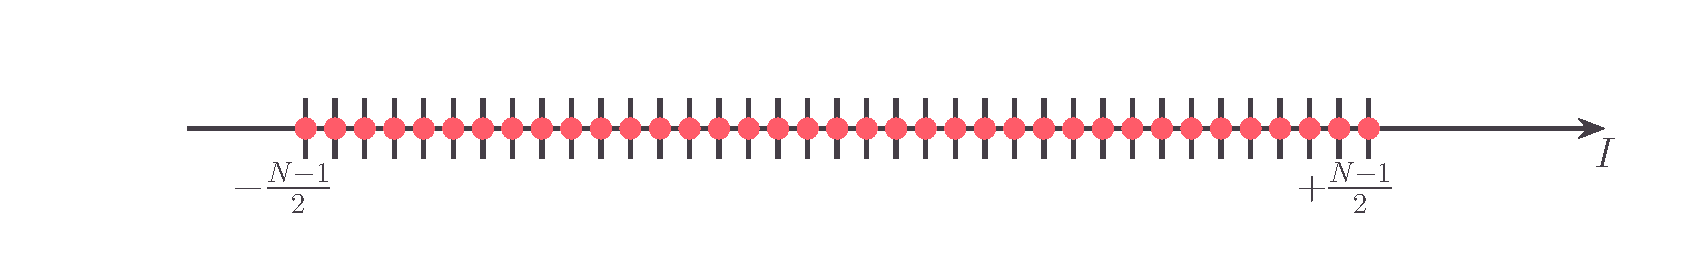
\includegraphics[width=1.5\textwidth , page = 1 ]{figures/Figures.pdf}  
      }   
    \end{column}
    \begin{column}{0.4\textwidth}
      \centering
      {\fontsize{6}{5}\selectfont  % <- ajuste ici aussi
      $$ \left \{ \begin{array}{rccl} L \rho(\theta) \delta \theta & : \# &  \mathrm{rapidities} &\in [\theta , \theta + \delta \theta ] \\ L \rho_h(\theta) \delta \theta & : \# &  \mathrm{holes} & \in [\theta , \theta + \delta \theta ] \\ L \rho_s(\theta) \delta \theta & : \# &  \mathrm{states} & \in [\theta , \theta + \delta \theta ]\end{array}\right . $$
      }
    \end{column}
  \end{columns}

\end{frame}

\Section{Large-scale dynamics}


\begin{frame}{Comparaison des commandes}
  \begin{itemize}
    \item<1-> \uncover<1->{\textbf{Uncover} : espace réservé}
    \item<2-> \visible<2->{\textbf{Visible} : sans espace réservé}
    \item<3-> \only<3->{\textbf{Only} : supprime l’élément avant}
    \item<4-> \onslide<4->{\textbf{Onslide} : garde l’espace}
    \item<5-> \alt<5>{\textcolor{red}{A}}{\textcolor{gray}{B}} : alterne contenu
  \end{itemize}
\end{frame}


% \begin{frame}
%   \frametitle{Rapidities and GGE in a classical system}
%   %\framesubtitle{Subtitle here}
  
%   \begin{columns}
%     \begin{column}{0.5\textwidth}
%       \begin{columns}
%       \begin{column}{0.5\textwidth} 
%       \centering
%       \animategraphics[
%         %controls,
%         %autoplay,     % démarre automatiquement
%         %loop,         % boucle infinie
%         width=0.7\linewidth,
%         %palindrome,       % (optionnel) rejoue à l'envers
%         buttonsize=1em,   % zone de clic autour
%         poster=first,     % affiche la première image au départ
%         %clicktoshow,      % permet de lancer/pause par clic
%         ]
%         {60}{figures/frames_2D_positions_animation/frame_}{00001}{00001}
%       \end{column}
%       \begin{column}{0.5\textwidth} 
%         \centering
%         \animategraphics[
%         %controls,
%         %autoplay,     % démarre automatiquement
%         %loop,         % boucle infinie
%         width=0.7\linewidth,
%         %palindrome,       % (optionnel) rejoue à l'envers
%         buttonsize=1em,   % zone de clic autour
%         poster=first,     % affiche la première image au départ
%         %clicktoshow,      % permet de lancer/pause par clic
%         ]
%         {60}{figures/frames_1D_positions_animation/frame_}{00001}{00001}
%         \animategraphics[
%         %controls,
%         %autoplay,     % démarre automatiquement
%         %loop,         % boucle infinie
%         width=0.7\linewidth,
%         %palindrome,       % (optionnel) rejoue à l'envers
%         buttonsize=1em,   % zone de clic autour
%         poster=first,     % affiche la première image au départ
%         %clicktoshow,      % permet de lancer/pause par clic
%         ]
%         {60}{figures/frames_1D_velocity_distribution/frame_}{00001}{0001} 
%       \end{column}
%       \end{columns}
%     \end{column}
%     \begin{column}{0.5\textwidth} 
%       \begin{columns}
%       \begin{column}{0.5\textwidth} 
%         \centering
%         \animategraphics[
%         %controls,
%         %autoplay,     % démarre automatiquement
%         %loop,         % boucle infinie
%         width=0.7\linewidth,
%         %palindrome,       % (optionnel) rejoue à l'envers
%         buttonsize=1em,   % zone de clic autour
%         poster=first,     % affiche la première image au départ
%         %clicktoshow,      % permet de lancer/pause par clic
%         ]
%         {60}{figures/frames_2D_velocity_distribution/frame_}{00001}{00001}
%       \end{column}
%       \begin{column}{0.5\textwidth} 
%         \centering
%       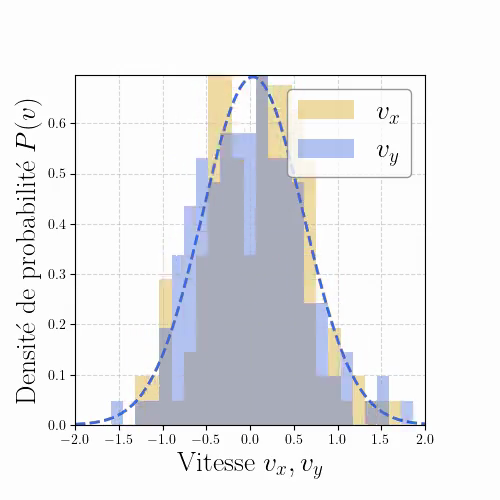
\includegraphics[width=0.8\linewidth]{figures/frames_2D_velocity_distribution/frame_00600.png}
%       \end{column}
%       \end{columns}
%     \end{column}
%   \end{columns}

% \end{frame}

% \begin{frame}
%   \frametitle{Rapidities and GGE in a classical system}
% \begin{columns}
%   \begin{column}{0.6\textwidth}
%     Colonne principale gauche
%     \begin{columns}
%       \begin{column}{0.5\textwidth}
%         Sous-colonne gauche
%       \end{column}
%       \begin{column}{0.5\textwidth}
%         Sous-colonne droite
%       \end{column}
%     \end{columns}
%   \end{column}
%   \begin{column}{0.4\textwidth}
%     Colonne droite
%   \end{column}
% \end{columns}
% \end{frame}

% \begin{frame}
%   \frametitle{Team}
%   %\framesubtitle{Subtitle here}
% % Clic sur l'image = play/pause (vidéo embarquée)
% \includemedia[
%   activate=onclick,
%   width=0.9\linewidth,
%   addresource=figures/1D_positions_animation.mp4,
%   transparent,
% ]{
\includegraphics{figures/frames_1D_positions_animation/frame_00001.png}}{figures/1D_positions_animation.mp4}
% \end{frame}

\Section{Demo}

\begin{frame}
  \frametitle{A frame with title and subtitle}
  \framesubtitle{Subtitle here}
  Lorem ipsum dolor sit amet, consectetur adipiscing elit, sed do eiusmod tempor incididunt ut labore et dolore magna aliqua \par
  Itemized list:
  \begin{itemize}
    \item Lorem ipsum
    \item Dolor sit amet
          \begin{itemize}
            \item Consectetur
            \item Adipiscing elit
          \end{itemize}
    \item Sed do eiusmod
          \begin{itemize}
            \item Tempor incididunt
                  \begin{itemize}
                    \item Ut labore et dolore
                    \item Magna aliqua
                  \end{itemize}
          \end{itemize}
  \end{itemize}
\end{frame}

\begin{frame}
  \frametitle{A frame with title only}
  \begin{theorem}
    \[e^{i\pi}+1=0\]
    \begin{proof}
      \begin{equation*}
        e^{iz}=\cos{z}+i\sin{z}
      \end{equation*}
      \center{therefore}
      \begin{align*}
        e^{i\pi}+1 & \null=\cos\pi+i\sin\pi+1 \\
                   & \null=-1+i\times0+1      \\
                   & \null=0
      \end{align*}
    \end{proof}
  \end{theorem}
\end{frame}

\begin{frame}[bg=demo-arguelles.png]
  \frametitle{A frame with background image}
  You can still add title and subtitle. \par
  You can also use a background in the title slide by setting: \\
  \texttt{\textbackslash frame[plain,bg=demo-background.jpg]\{\textbackslash titlepage\}}
\end{frame}

\begin{frame}[plain]
  \frametitle{A plain frame has no headline}
  \begin{table}
    \small
    \begin{tabular}{rl}
      \ttfamily\textbackslash Alegreya              & \Alegreya Lorem ipsum dolor sit amet              \\
      \ttfamily\textbackslash AlegreyaMedium        & \AlegreyaMedium Lorem ipsum dolor sit amet        \\
      \ttfamily\textbackslash AlegreyaExtraBold     & \AlegreyaExtraBold Lorem ipsum dolor sit amet     \\
      \ttfamily\textbackslash AlegreyaBlack         & \AlegreyaBlack Lorem ipsum dolor sit amet         \\
      \ttfamily\textbackslash AlegreyaSansThin      & \AlegreyaSansThin Lorem ipsum dolor sit amet      \\
      \ttfamily\textbackslash AlegreyaSansLight     & \AlegreyaSansLight Lorem ipsum dolor sit amet     \\
      \ttfamily\textbackslash AlegreyaSans          & \AlegreyaSans Lorem ipsum dolor sit amet          \\
      \ttfamily\textbackslash AlegreyaSansMedium    & \AlegreyaSansMedium Lorem ipsum dolor sit amet    \\
      \ttfamily\textbackslash AlegreyaSansExtraBold & \AlegreyaSansExtraBold Lorem ipsum dolor sit amet \\
      \ttfamily\textbackslash AlegreyaSansBlack     & \AlegreyaSansBlack Lorem ipsum dolor sit amet
    \end{tabular}
  \end{table}
  \vfill
  \begin{alert}{Alert!}
    A \textit{plain} frame does not show the progress bar but still appears in it unless the frame comes after \texttt{\textbackslash End}
  \end{alert}
\end{frame}

\begin{frame}[standout]
  \centering\large
  A \textbf{\itshape\scshape standout} frame can be used to focus attention
\end{frame}

\End
\begin{frame}[plain,standout]
  \centering
  In combination with \textit{plain}, \\
  it makes a nice thank-you slide!
  \vfill
  \scalebox{4}{\faGithub} \par\bigskip
  \url{https://github.com/piazzai/arguelles} \\
  \url{https://ctan.org/pkg/beamertheme-arguelles}
\end{frame}

\end{document}
